\section{Monolayer Preparation}

\begin{comment}
In this section we explain about our experimental procedure. This experiment had two parts of the proceddure, namely, sample making and measurement contact angle of samples to evaluate the quality of sample and identify the thiol. 
first part, we made SAM and this procedure was adapted from Sigma-Aldrich.
\end{comment}

One of the most widely studied systems of SAMs are gold-alkylthiolate monolayers(Fig. \ref{fig:sam1}), in this experiment we used this method.
In general, adsorption is performed in 10–1000 mM solutions of thiols, dithiols,
dialkyldisulfides (in general S–S bonds break upon adsorption and thiolate SAMs are obtained) and dialkylsulfides in different solvents, depending on the nature of the molecule. Mixed monolayers may be formed if the solution contains two or more different thiols.

Each of the molecules that constitute the building blocks of the system can be
divided into three different parts (Fig. \ref{fig:sam2}):
the head-group (linking group), the backbone (main chain), and the specific terminal (active) group. The head-group guides the self-assembly process on each type of substrate, linking the hydrocarbon chain (of variable length) to the metal surface through a strong bond.
The interactions among backbone hydrocarbon chains (involving van der Waals and hydrophobic forces) ensure an efficient packing of the monolayer and contribute to stabilize the structures with increasing chain length.
The terminal group confers specific properties to the surface (hydrophilic, hydrophobic), and can also be used to anchor different molecules, biomolecules, or nanostructures by weak interactions or covalent bonds.


\begin{figure}[h]
\centering
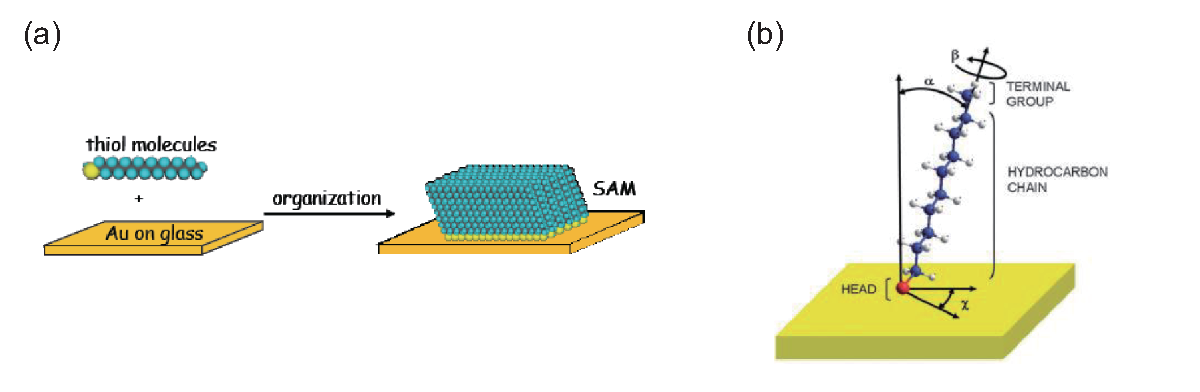
\includegraphics[width=0.6\columnwidth]{sam.eps}
\caption{Formation of a SAM on a gold surface via sulfide bridges.}
\label{sam1}
\end{figure}

\begin{figure}[h]
\centering
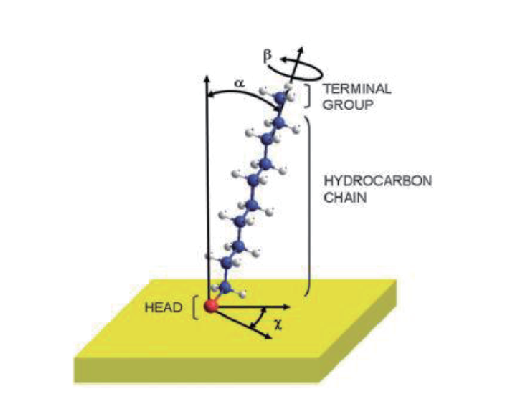
\includegraphics[width=0.6\columnwidth]{sam2.eps}
\caption{Formation of a SAM on a gold surface via sulfide bridges.}
\label{sam2}
\end{figure}


\subsection{Determine necessary amounts and concentration of thiol solution}

We calculated the total volume of thiol solution needed to make the number of samples desired and the total amount of thiol needed to prepare desired amount of thiol solution. We used a powder chemical reagent (204.37 g/mol) and a liquid chemical reagent ($138.23 \ {\rm g/mol}$ and $1.032 \ {\rm g/mL})$, respectively. 

Mass of thiole is given by 
$ {\rm Total\ volume \times Consentration \times Molecular \ Weight}$, namely,

\begin{equation}
 m\, [{\rm g}]=V \, [{\rm l}] \cdot c \, \left[ \frac{{{\rm mol}}}{\rm l}\right] \cdot 
\text{Molecular Weight} \left[ \frac{\rm g}{{\rm mol}}\right]
\end{equation}
Where MW is the Molecular Weight of the thiol, and c is the concentration.
In this time we would make a thiol solution for 10 mL with 1 mil mol/L, so the prepared mass of tiole is 
\begin{eqnarray}
m\, [{\rm g}]=10\times 10^{-3}\cdot 1\times 10^{-3} 
\cdot  204.37  \nonumber
=204.37 \times 10^{-5} \, {\rm g}
\end{eqnarray}

Similarly, the prepared liquid volume of thiol is
\begin{eqnarray}
 l\, [{\rm l}] &=& V \, [{\rm l}] \cdot c , \left[ \frac{{{\rm mol}}}{\rm l}\right] \cdot 
\frac{\rm Molecular \ Weight}{\rm Density} \left.  \left[ \frac{\rm g}{{\rm mol} }\right/\frac{\rm g}{\rm l}\right] \nonumber \\
& =& 10\times 10^{-3}\cdot 1\times 10^{-3} \cdot  \frac{138.23}{1.032\times 10^{3}} \nonumber \\
&=& 133.944 \times 10^{-8} \, {\rm l} \simeq 1.3 \, \mu \rm l
\end{eqnarray}

Therefore, we prepared a powder for $204.37 \times 10^{-5} \, \rm g$ measuring by an electronic scale and a liquid for $1.3 \, \mu  \rm l$ measuring by a micropipette, respectively.



\subsection{Prepare Thiol Solution}
\begin{enumerate}
 \item First of all, we cleaned all laboratory apparatus, namely, beakers, tweezers and so on with ethanol for 2-3 times.


 \item We prepared 3 gold coated substrates for the base of SAM and cleaned them by an ultrasonic bath for 10 minutes with 37 kHz.
 \item We dispense the mass and volume of thiol into the solvent and made two tipys of thiol solutions with 1 mil mol/l for 10 ml. We sonicated these solutions for 3 minutes to dissolve.
 \item After dissolved, we dispensed the $3 \, \mu \rm l$ solutions into each sample containers. Therefore we made 3 kinds of solutions, or one was the solution made by a powder thiol reagent, another was by a liquid thiole reagent, and the other was mixed the above two ones equally. 
\end{enumerate}
%%%%%%%%%%%%%%%%%%%%%%
\subsection{Sample Self-Assembly}
\begin{enumerate}
 \item We immersed 3 gold sbstrates into 3 sample containers, respectively.  
%\end{enumerate}
%\subsection{Sample S}
%\begin{enumerate}
 \item We placed the samples in clean petri dish individually and backfilled petri dishes with dry nitrogen to avoid oxidized. We attached the container mouth part firmly with parafilm and stored them in a fume hood. They would be kept for around 24 hours to grow up better quality samples.
\end{enumerate}
So, we finished to set up our samples. And hereafter we used samples from the previous group to continue the process.


\subsection{Terminate Self-Assembly}
After took the samples out from the cases we rinsed with solvent and dried them with nitrogen gas. Then we sonicated the samples for 10 minutes with ethanol. The frequency is 37 kHz with 50 \% and dried them with a stream of dry nitrogen. The samples was completely prepared.


